% 村松先生向け 基本スライド（日本語）
%
% ビルド: lualatex slides_muramatsu_ja.tex   （2回）
%   luatexja は TeX Live のフル導入に標準で入っています。既定の日本語フォント
%   （原ノ味）が無い環境では 1 行目付近の \usepackage{luatexja} を
%   \usepackage[ipaex]{luatexja-preset} などに差し替えてください。
%
% 必要パッケージ: luatexja（Debian/Ubuntu なら texlive-lang-japanese、
%   加えて texlive-luatex / texlive-latex-extra）。
%   ビルド確認済み: 9 ページ、エラー 0、Overfull 0。
%
% CONSTRAINT: 基本スライド。10 ページ以内に収める。増やすなら何かを削る。
%
% 構成の方針: 「何をしたか」の羅列ではなく、
%   (1) 鎖のどこを担当したか  (2) 各主張の根拠と、その強さ
% の2点を骨格にする。研究室内の発表なので、確かさの段階を明示することを優先。
\documentclass[aspectratio=169,11pt]{beamer}
\usepackage{luatexja}
\usetheme{Madrid}
\usecolortheme{seahorse}
\usepackage{booktabs}
\usepackage{amsmath,amssymb}
\usepackage{bm}
\usepackage{xcolor}
\usepackage{graphicx}
\usepackage{tikz}
\usetikzlibrary{shapes.geometric,arrows.meta,positioning,fit,backgrounds,calc}

\definecolor{c3}{RGB}{30,80,160}
\definecolor{cok}{RGB}{30,120,60}
\definecolor{cwarn}{RGB}{190,110,20}
\definecolor{copen}{RGB}{190,40,40}
\setbeamercolor{frametitle}{bg=c3, fg=white}
\newcommand{\lv}[2]{\textcolor{#1}{\textbf{#2}}}

\title{口腔バイオフィルムの成長応力解析}
\subtitle{修士論文の現状と，村松研で継続する部分}
\author[西岡佳祐]{西岡佳祐}
\institute[IKM, LUH / 慶應]{%
\small ライプニッツ大学ハノーファー 連続体力学研究所（IKM）\\
\small 慶應義塾大学}
\date{2026年10月}

\begin{document}
\maketitle

% --------------------------------------------------------
\begin{frame}{お話しする順番}
\begin{enumerate}\small
  \item \textbf{位置づけ} —— 研究全体の鎖のうち、修論はどこを担当するか
  \item \textbf{作ったもの} —— ANSYS の材料サブルーチン
  \item \textbf{確かさ} —— 各主張の根拠と、その強さ（ここが中心）
  \item \textbf{結果} —— 4つの臨床条件で応力がどう変わるか
  \item \textbf{未解決} —— 説明できていないこと
  \item \textbf{村松研で継続する部分} —— 温存している研究項目
\end{enumerate}
\vspace{8pt}
{\footnotesize 方針として、「動いた」と「確かめた」を分けて書いています。
確かめていないことを確かめたように書かないほうが、後で効くと考えています。}
\end{frame}

% --------------------------------------------------------
\begin{frame}{1. 位置づけ：研究全体の鎖と、修論の担当範囲}
\vspace{2pt}
\begin{center}
\begin{tikzpicture}[
  node distance=3mm, font=\scriptsize,
  box/.style={draw, rounded corners=2pt, align=center, minimum height=9mm,
              text width=19mm, fill=gray!8},
  mine/.style={box, fill=c3!18, draw=c3, very thick},
  ar/.style={-{Stealth[length=2mm]}, gray}]
  \node[box] (a) {CLSM で測った\\菌種組成};
  \node[box, right=of a] (b) {TMCMC で較正\\5種生態モデル};
  \node[box, right=of b] (c) {成長場\\$\alpha(x)$};
  \node[mine, right=of c] (d) {FEM 材料則\\$\bm{F}_g=(1{+}\alpha)\bm{I}$};
  \node[mine, right=of d] (e) {von Mises 応力\\条件間比較};
  \foreach \i/\j in {a/b, b/c, c/d, d/e} \draw[ar] (\i) -- (\j);
  \node[below=6mm of d, font=\scriptsize, text=c3] (lab)
       {\textbf{修論（IKM 提出版）の本体}};
  \draw[c3, thick, rounded corners]
       ($(d.north west)+(-1mm,1mm)$) rectangle ($(e.south east)+(1mm,-1mm)$);
\end{tikzpicture}
\end{center}
\vspace{2pt}
\begin{itemize}\small
  \item 左の2つ（組成データ・生態モデル）は既にあるものを使う側
  \item 修論は\textbf{右の2つ}：生態の出力を FEM に入れて応力にする部分
  \item 生態モデル自体の発展は、来年度 村松研で継続する予定
\end{itemize}
\end{frame}

% --------------------------------------------------------
\begin{frame}{2. 作ったもの：ANSYS の材料サブルーチン（USERMAT）}
\small 成長と粘弾性を持つ構成則を、ANSYS が要素ごとに呼ぶ材料ルーチンとして実装。
\vspace{4pt}
\begin{itemize}\small
  \item 成長運動学 $\bm{F}=\bm{F}_e\bm{F}_v\bm{F}_g$、$\bm{F}_g=(1+\alpha)\bm{I}$
  \item 接線剛性は $\bm{F}$ 摂動による数値微分（閉形式ではない）
  \item ANSYS の include も common block も使わない自己完結型
        $\Rightarrow$ \textbf{ANSYS のバージョンに依存しない}
  \item 共同研究先（ハノーファーの Oliver 氏）のフレームワークの
        呼び出し点に、そのまま差し込める形にしてある
\end{itemize}
\vspace{4pt}
{\footnotesize 移植で最も事故が起きやすいのは Voigt 順序で、
ANSYS と Abaqus でせん断成分の並びが違います。
そのため2つの実装でインデックス写像は共有できません。}
\end{frame}

% --------------------------------------------------------
\begin{frame}{3. 確かさ：主張と、その根拠（ここが中心）}
\vspace{-1pt}
\begin{center}\scriptsize
\begin{tabular}{p{3.5cm}p{4.6cm}l}
\toprule
主張 & 根拠 & 強さ \\
\midrule
2つの実装が同じ式を計算している &
独立に書いた Abaqus UMAT と 8017 状態で一致（ビット単位） &
\lv{cok}{0 ULP} \\[2pt]
成長運動学が正しく組めている &
自由膨張は応力ゼロ、完全拘束は解析解。ANSYS の印字全桁で一致 &
\lv{cok}{閉形式} \\[2pt]
実ソルバーで収束する &
12240 要素、各サブステップ 1--4 反復。自動時間刻みは一度も縮めず拡大 &
\lv{cok}{実機} \\[2pt]
成長変数が壊れずに往復する &
状態スロット 176{,}800 サンプルすべて書いた値のまま &
\lv{cok}{実機} \\[2pt]
生態系モデルが論文どおり &
Klempt et al.\ 2026 の数値例 14 件をすべて再現（誤植 2 か所も特定） &
\lv{cok}{外部} \\[2pt]
式そのものが正しい &
\textbf{言えない}。等容分解の $J^{-2/3}$ に不整合を発見 &
\lv{cwarn}{限界に明記} \\
\bottomrule
\end{tabular}
\end{center}
\vspace{3pt}
{\footnotesize 最下行が要点です。2実装が一致しても「式が正しい」ことは言えません。
実際に不整合があり、影響は\textbf{純粋に静水圧成分のみ}で
報告している von Mises には効かないことを確かめた上で、限界として章に書いています。}
\end{frame}

% --------------------------------------------------------
\begin{frame}{4. 結果：4つの臨床条件（接着バグ修正後に再計算）}
\small 実測の Day-1 CLSM 組成を4条件ぶん与え、曲面シェル上で解いた。
\vspace{4pt}
\begin{center}\small
\begin{tabular}{@{}lcc@{}}
\toprule
 & 以前の報告 & \textbf{修正後} \\
\midrule
成長層 / 基材の von Mises & $15.2$ 倍 & $\mathbf{6.3}$ \textbf{倍} \\
条件間の応力の広がり & $9.1\%$ & $\mathbf{0.4\%}$ \\
条件間の成長 $\alpha$ の幅 & $1.106$ 倍 & $1.006$ 倍 \\
\bottomrule
\end{tabular}
\end{center}
\vspace{4pt}
\begin{itemize}\small
  \item 応力は荷重ではなく\textbf{成長機構}が作っている点は変わらず
  \item ANSYS の $\alpha$ は独立な参照計算と全積分点で一致
\end{itemize}
\vspace{4pt}
\begin{center}
\colorbox{cwarn!12}{\parbox{0.93\linewidth}{\footnotesize
\textbf{以前の数字は誤りでした。}基材と成長層を \texttt{NUMMRG}（一致する節点だけ結合）で
つないでいたため、この計算では\textbf{角の4節点しか接着されていません}でした。
\texttt{VGLUE} で界面を共有させて修正し、メッシュ収束（2次）を確認。定数も TMCMC の
校正条件（$c^*=25$、Hill なし、$\alpha^*=0$）に統一しました。
対の計算も再計算した結果、置き場所・隣接領域の影響が最大 0.28\% と条件間の差と同程度で、
「条件が応力を動かす」という以前の結論は取り下げます。}}
\end{center}
\end{frame}

% --------------------------------------------------------
\begin{frame}{5. なぜ条件で応力が変わらないか（モデルの定義から）}
\begin{center}
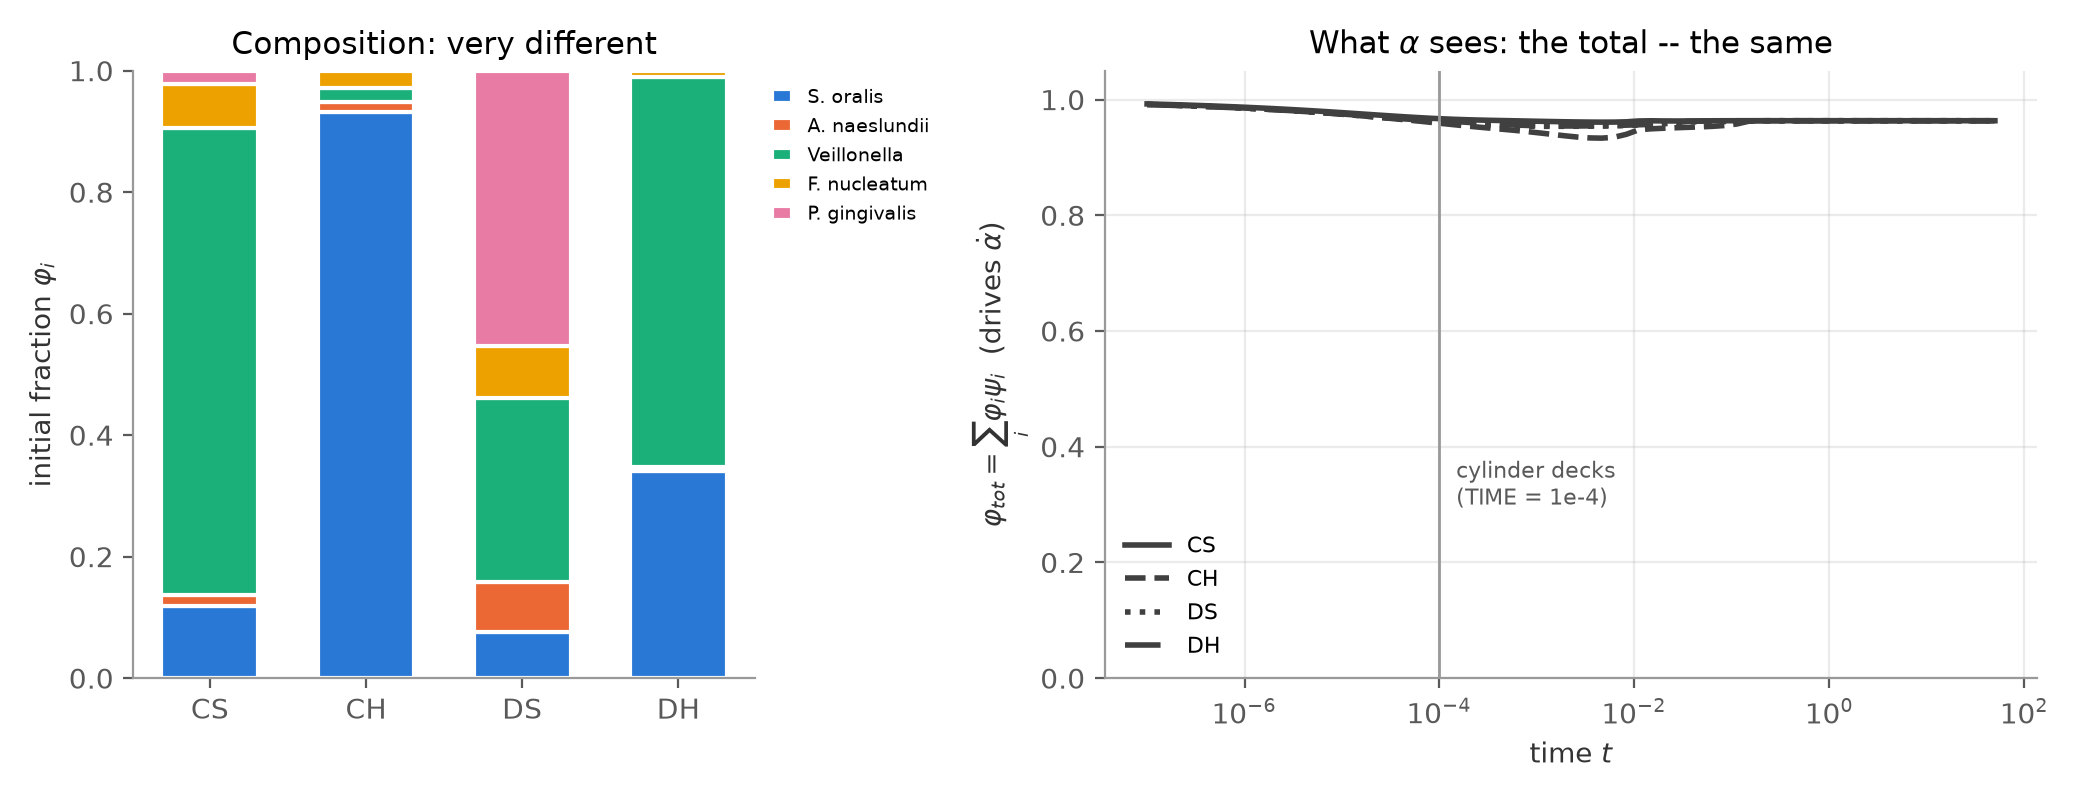
\includegraphics[width=0.72\linewidth]{assets/condition_total_phi.png}
\end{center}
\vspace{-6pt}
\begin{itemize}\footnotesize
  \item 条件が応力に届く経路は $\alpha$ だけ（物性は全領域で同一）。
        $\dot\alpha = k_\alpha\,\varphi_{\mathrm{tot}}$、
        $\varphi_{\mathrm{tot}}=\sum_i\varphi_i\psi_i$ は\textbf{合計}しか見ない
  \item CLSM 組成は割合なので全条件 $\sum_i\varphi_i=1$ から出発し、
        同じ値（0.9635）に収束 $\Rightarrow$ \textbf{組成の違いは足し算で消える}
  \item 成長時間を延ばしても差は開かず、むしろ閉じる
  \item 残る約 0.5\% の差も、生態の時間刻みを細かくすると\textbf{条件の順位が入れ替わる}
\end{itemize}
\vspace{2pt}
{\footnotesize 以前「1条件だけ約5\%外れる」と書いた未解決点は、接着修正後の再計算で消えました。
組成を応力に届かせるには、菌種別の成長率・絶対量（割合でなく）・組成依存の剛性のいずれかが必要です。}
\end{frame}

% --------------------------------------------------------
\begin{frame}{6. 村松研で継続する部分（2026-06-29 時点）}
\small 修論本体には収録せず、継続研究として温存しているもの。
\vspace{2pt}
\begin{center}\scriptsize
\begin{tabular}{llp{5.3cm}}
\toprule
ID & 内容 & 状況 \\
\midrule
A & 成長 Jacobian $\partial\sigma/\partial\varphi_i$ & \lv{cok}{実装済み}。機構的感度の議論に育てる \\
B & AT2 フェーズフィールド破壊 & \lv{cok}{実装済み}。$t_{\mathrm{crit}}$ と生態の結合（橋渡しは実装済み） \\
D & 2チャンネル粘弾性 UMAT & \lv{cok}{実装済み}。時間依存性が要るなら条件スイープ \\
C$'$ & Replicon 安定性解析（disordered-gLV） & \lv{cok}{実装済み}。小規模群集のディスバイオシス様式を執筆 \\
C & 状態依存 $A_{ij}$ の分岐 & \lv{copen}{未着手}。\textbf{データ量が律速} \\
E & Neural PDE サロゲート & \lv{copen}{未着手}。低優先（速度のみ、直接解法で足りる） \\
F & J 積分 $G_c$ 後処理 & \lv{copen}{未着手}。B で代替可 \\
\bottomrule
\end{tabular}
\end{center}
\vspace{4pt}
{\footnotesize A・B・D・C$'$ は動くところまで到達しています。
C は手法ではなくデータが律速で、E・F は優先度が低いと判断しています。}
\end{frame}

% --------------------------------------------------------
\begin{frame}{一番有望だと考えている継続テーマ}
\vspace{4pt}
\begin{center}
\colorbox{c3!12}{\parbox{0.9\linewidth}{\centering\small
\textbf{生態と力学の橋渡し}\\[3pt]
ディスバイオシスは生態学的には安定性を限界まで下げるのに、\\
力学的には破壊が\textbf{遅くなる}\\[3pt]
—— 生態学的安定性と力学的堅牢さのトレードオフ}}
\end{center}
\vspace{6pt}
\begin{itemize}\small
  \item 橋渡しの実装は既にある（replicon 側と AT2 側をつなぐ）
  \item 機構として新しく、論文になりうると考えている
  \item 自然な深掘りは C（状態依存の相互作用）だが、\textbf{データ待ち}
\end{itemize}
\end{frame}

% --------------------------------------------------------
\begin{frame}{当面の予定と、ご相談したいこと}
\begin{itemize}\small
  \item \textbf{11月下旬}：修士論文 提出（IKM）\quad
        \textbf{12月}：口頭試問
  \item 修論は FEM 材料則の寄与に絞る。JAXFEM で書いていた部分は
        \textbf{慶應での継続のために温存}する方針
\end{itemize}
\vspace{8pt}
\begin{center}
\colorbox{c3!10}{\parbox{0.9\linewidth}{\small
\textbf{ご相談したいこと}
\begin{enumerate}\footnotesize
  \item 「今のモデルでは組成は応力に効かない」を修論の結論としてよいか。
        組成を効かせる経路（5.）は将来課題でよいか
  \item 継続テーマとして上記の方向で問題ないか
  \item C（状態依存 $A_{ij}$）に必要なデータの見通し
  \item 単位互換・ダブルディグリーの手続き
\end{enumerate}}}
\end{center}
\end{frame}

\end{document}
